\documentclass[11pt]{article}

\author{Math 123}
\date{Due March 10, 2023 by midnight} 
\title{Homework 6}

\usepackage{graphicx,xypic}
\usepackage{amsthm}
\usepackage{amsmath,amssymb}
\usepackage{amsfonts}
\usepackage{xcolor}
\usepackage[margin=1in]{geometry}
\usepackage[shortlabels]{enumitem}
\newtheorem{problem}{Problem}
\renewcommand*{\proofname}{{\color{blue}Solution}}


\usepackage{fancyhdr}
\pagestyle{fancy}
\rhead{Math 123, Homework 6}

\setlength{\parindent}{0pt}
\setlength{\parskip}{1.25ex}


\begin{document}

\maketitle

% You are required to put your name here:
{\bf\Large Name:} 


\vspace{.3in}
Topics covered: vertex cuts, connectivity, Menger's theorem, network flows

Instructions: 
\begin{itemize}
\item This assignment must be submitted on Gradescope by the due date. 
\item If you collaborate with other students (which is encouraged!), please mention this somewhere on the assignment. 
\item If you are stuck, please ask for help (from me, a TA, a classmate). Use Campuswire!  
\item You may freely use any fact proved in class. In general, you should provide proof for facts used that were not proved in class. 
\item Please restrict your solution to each problem to a single page. Usually solutions can be even shorter than that. If your solution is very long, you should think more about how to express it concisely.
\end{itemize}

\pagebreak 


\begin{problem}
Let $G$ be a graph. 
\begin{enumerate}[(a)]
\item Give a counterexample to the following statement: If $e$ is a cut-edge of $G$, then at least one vertex of $e$ is a cut-vertex of $G$. \footnote{We did not define cut edge in class, but it means what you most likely guess.} 
\item Add a hypothesis to correct the above statement. 
\end{enumerate} 
\end{problem}

\begin{proof}

\end{proof}

\pagebreak
\begin{problem}
Compute (with proof) $\kappa(u,v)$ for the graph below.
\begin{center}
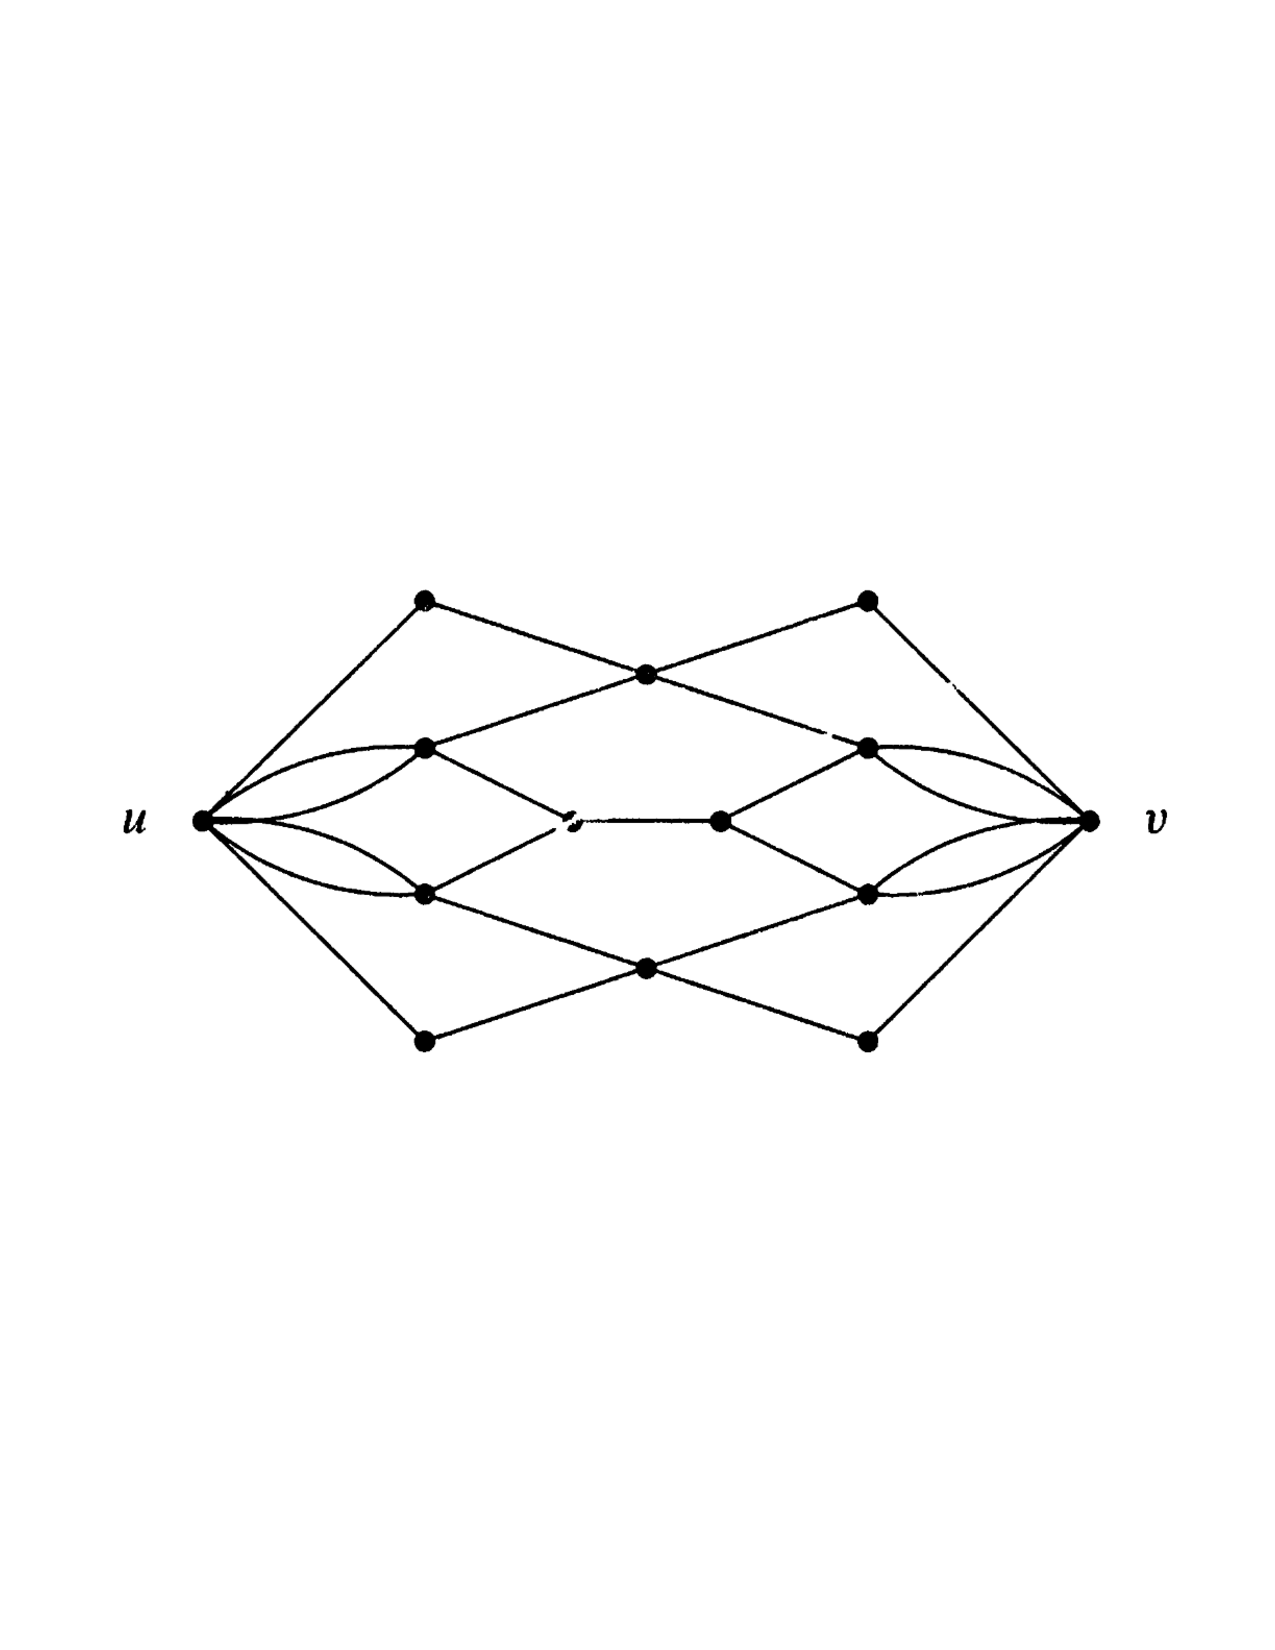
\includegraphics[scale=.4]{hw6-graph.pdf}
\end{center}
\end{problem}

\begin{proof}

\end{proof}

\pagebreak
\begin{problem}
Find (with proof) the smallest $3$-regular graph with $\kappa(G)=1$. \footnote{Hint: consider a 1-element vertex cut $S$. What does $G\setminus S$ look like? } 
\end{problem}

\begin{proof}

\end{proof} 


\pagebreak
\begin{problem}
Fix $k\ge2$ and let $Q_k$ be the hypercube graph. Prove that for any pair of vertices $x,y$ there exist $k$ pairwise disjoint $(x,y)$-paths. 
\end{problem}

\begin{proof}

\end{proof}

\pagebreak
\begin{problem}
Use Menger's theorem to prove K\"onig's theorem: if $G=(X\sqcup Y,E)$ is bipartite the maximum size of a matching of $G$ is equal to the minimum size of a vertex cover of $G$. \footnote{Hint: consider graph $G'$ obtained by adding vertices $a,b$ to $G$ and connecting $a$ to every vertex of $X$ and $b$ to every vertex of $Y$. } 
\end{problem}

\begin{proof}

\end{proof}


\pagebreak
\begin{problem}
Use the matrix-tree theorem\footnote{From the end of lecture 2/28} to prove Cayley's theorem.\footnote{Use a connection between the determinant and eigenvalues. It may help to first try to guess the form of the answer. For the love of algebra, do NOT compute any determinants!}
\end{problem}

\begin{proof}

\end{proof} 


\end{document}